\documentclass[a4paper]{scrartcl}
\usepackage{amsmath}
\usepackage{mathtools}
\usepackage[utf8]{inputenc}
\usepackage[polish]{babel}
\usepackage{textcomp}
\usepackage[T1]{fontenc}
\usepackage{amsthm}
\usepackage{amsfonts}
\newtheorem{definition}{Definicja}
\newtheorem{theorem}{Twierdzenie}
\newtheorem{lemma}{Lemat}
\usepackage{hyperref}
\hypersetup{
    colorlinks,
    citecolor=black,
    filecolor=black,
    linkcolor=black,
    urlcolor=black
}
\usepackage{algorithmic}
\title{Algorytmy i struktury danych}
\subtitle{Zadanie 9, lista 2}
\author{Dawid Żywczak}
\date{24 kwietnia 2020}

\begin{document}
\maketitle
Do rozwiązania problemu postawionego w zadaniu skorzystamy z kodowania Huffmana, gdzie symbolami będą nasze liście, natomiast częstości występowania to wartości $w_1, w_2,...,w_n$. Przedstawię teraz algorytm, a następnie lematy, które pomogą w udowodnieniu poprawności rozwiązania. Algorytm wygląda następująco:
\begin{algorithmic}
\STATE $Q\gets$ kolejka priorytetowa liści
\FOR{$i=1$ \TO $i=n-1$ } 
	\STATE stwórz nowy węzeł v
	\STATE ustaw lewe dziecko v na deletemin(Q)
	\STATE ustaw prawe dziecko v na deletemin(Q)
	\STATE przypisz wagę v jako suma wag jego dzieci
	\STATE dodaj v do Q
\ENDFOR
\end{algorithmic}
(niżej indeks 1 oznacza drzewo T, indeks 2 oznacza drzewo $T'$)
\begin{lemma}
Dowolny wierzchołek w optymalnym drzewie, rozwiązującym problem z zadania, posiada dwóch synów lub jest liściem.
\end{lemma}
\begin{proof}
Załóżmy niewprost, że istnieje drzewo optymalne T, które posiada wierzchołek mający tylko jednego syna, nazwijmy ten wierzchołek v. Rozważmy drzewo $T'$ powstałe przez usunięcie wierzchołka v i ``podłączenie`` jego jedynego poddrzewa w jego miejsce. Teraz zauważmy, że w wyniku usunięcia wierzchołka v, $EL(T) > EL(T')$, a zatem T nie jest optymalnym rozwiązaniem, sprzeczność.
\end{proof}
\begin{lemma}
Jeśli wierzchołki a i b są liśćmi o najmniejszej wadze, to istnieje drzewo optymalne T, w którym a i b są braćmi.
\end{lemma}
\begin{proof}
Weźmy optymalne drzewo T, załóżmy że liście c i d są braćmi. Niech L będzie zbiorem liści drzewa T. Pokażemy, że możemy zamienić drzewo T na inne, lepsze drzewo $T'$ w którym a i b są braćmi. 
\begin{center}
	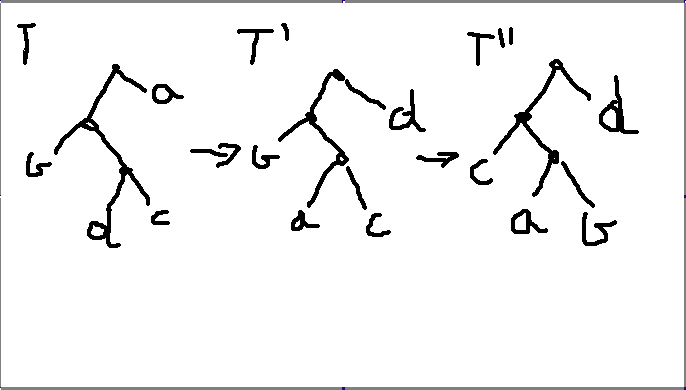
\includegraphics[scale=0.2]{przejscia.png}
\end{center}
Bez starty ogólności załóżmy, że $c(d) \leq c(c)$ i $c(a) \leq c(b)$. Oczywiście też $c(a) \leq c(d)$ i $c(b) \leq c(c)$. Prześledźmy jak działa przejście z T do $T'$. Zamieniami wierzchołek d z wierzchołkiem c miejscami, w wyniku czego otrzymujemy drzewo o mniejszej wadze EL. Zobaczmy dlaczego.
\begin{center}
$EL(T) - EL(T') = \sum_{v \in L} c(v)\cdot d_1(v) - \sum_{v \in L'}c(v) - d_2(v) = c(a)d_1(a) + c(d)d_1(d) - c(a)d_2(a) - c(d)d_2(d) = c(a)d_1(a) + c(d)d_1(d) - c(a)d_1(d) - c(d)d_1(a) = (c(d) - c(a))(d_1(d) - d_1(a)) \geq 0$
\end{center}
Analogicznie możemy pokazać dla przejścia $T'$ w $T''$, a skoro T jest optymalne to $T'$ też.
\end{proof}
\begin{lemma}
Niech a i b będą liśćmi o najmniejszej wadze. Niech d będzie nowym wierzchołkiem o $c(d) = c(a) + c(b)$ i niech $L' = L \setminus \{a, b\} \cup \{d\}$ (d wstawiamy w miejsce ojca a i b). Wtedy jeśli $T'$ jest optymalnym drzewem dla $L'$ to T jest optymalne dla L.
\end{lemma}
\begin{proof}
Zauważmy najpierw, że wagi wierzchołków których nie zmieniami są takie same w drzewie T i $T'$. Zauważmy też, że $d_1(a) = d_1(b) = d_2(d)+1$. Wtedy
\begin{center}
$c(a)d_1(a) + c(b)d_1(b) = (c(a) + c(b))(d_2(d) + 1) = c(a) + c(b) + (c(a) + c(b))d_2(d) = c(a) + c(b) + c(d)d_2(d)$.
\end{center}
Czyli $EL(T) = EL(T') + c(a) + c(b)$. Załóżmy, że $T'$ jest optymalne, ale T nie jest. Istnieje zatem drzewo G t.że $EL(G) < EL(T)$ (T i G mają ten sam zbiór liści). Zamieńmy teraz parę liści a i b o tym samym ojcu (wiem, że taka para istnieje z lematu 1.) na wierzchołek d, taki że $c(d) = c(a) + c(b)$. Korzystając z równania znajdującego się wyżej, wiem że otrzymujemy drzewo o wadze $EL(G) - c(a) - c(b) < EL(T) - c(a) - c(b) = EL(T')$ co jest sprzeczne z optymalnością $T'$.
\end{proof}
Uzbrojeni w te wszystkie lematy, możemy przejść do dowodu poprawności algorytmu. Zrobimy to indukcyjnie po mocy zbioru liści.
\begin{proof}
Baza: 1 liść - z lematu 1. drzewo jednoelementowe
2 liście - oczywiste
Krok: Załóżmy, że nasz algorytm znajduje optymalne rozwiązanie dla $\|L\|\leq n$. Weżmy zbiór $L'$ o mocy $n+1$. Wybierzmy dwa wierzchołki o najmniejszej wadze, będące braćmi oraz nazwijmy je a i b. Zastąpmy je wierzchołkiem d tak jak w lemacie 3. Otrzymujemy zbiór liści o mocy $n$ więc z założenia potrafimy znaleźć dla niego rozwiązanie optymalne $T'$. Teraz niech a i b będą synami wierzchołka d. Wtedy z lematu drugiego wiemy, że drzewo otrzymane w ten sposób jest optymalnym rozwiązaniem dla zbioru $L'$.
\end{proof}
Złożoność czasowa: Budujemy na początku kolejkę, co zajmuje nam O(n), później w każdym przebiegu pętli usuwamy dwa razy min oraz wrzucamy jeden element na kopiec. Otrzymujemy zatem O(nlogn).\\
Złożoność pamięciowa: O(n) - musimy trzymać kolejkę w pamięci
\end{document}